\chapter{Basic Definitions and Theorems}

\section{Path-connectedness and Homotopy}

\begin{defn}[Path]
    Given any points $x,y$ in a topological space $X$, a path in $X$ from $x$ to $y$ is a continuous function $\alpha : [0,1] \lra X$ with $\alpha(0) = x$ and $\alpha(1) = y$, since we can rescale it to $\beta(t) = \alpha((b-a)t + a)$ for $t \in [0,1]$
\end{defn}
\begin{defn}[Path-connectedness]
    A path connected space is a topological space $X$ in which for any points $x,y \in X$ there exists a path in $X$ from $x$ to $y$.
\end{defn}

\begin{defn}[Homotopy]
Let $X$ and $Y$ be two topological spaces, let $f,g : X \lra Y$ be maps and $I = [0,1]$. Then the \textit{homotopy} from $f$ to $g$ is the map $F: X \times I \lra Y$ such that $F(x,0) = f(x)$ and $F(x,1) = g(x)$ for all points $x \in X$.
\end{defn}

\begin{notn}
If $F$ is the homotopy from $f$ to $g$ we write $\disp f \htp{F} g.$
\end{notn}

If in addition, $f$ and $g$ agree on some subset $A$ of $X$, we may wish to deform $f$ to $g$ without altering the values of $f$ on $A$. IN this particular case, we define an homotopy $F$ from $f$ to $g$ with the additional property that 
\[
    F(a,t) = f(a) \quad \text{for all $a \in A$, and all $t \in I = [0,1]$}  
\]
when such homotopy exists we say that $f$ is homotopic to $g$ relative to $A$.

\begin{notn}
    If $F$ is the homotopy from $f$ to $g$ relative to $A$ we write $\disp f \htp{F} g \rel A.$
\end{notn}

\subsection*{Examples os homotopy}
\begin{enumerate}
    \item If $f,g : \RR \ra \RR^2$ are given by $f(x) = (x, x^3)$ and $g(x) = (x, e^x)$, then the map $H : \RR \times [0,1] \ra \RR^2$ given by 
    \[
        H (x,t) = \left(x, (1-t)x^3 + te^x\right) 
    \]
    is a homotopy between them.
    \item Suppose $C \subseteq \RR$ is a convex subset of Euclidean space and $f,g : [0,1] \ra C$ are paths with the same endpoints, then there is \textit{straight line homotopy} given by
    \begin{align*}
        H : [0,1] \times [0,1] & \lra C \\
        (s,t) & \mapsto (1-t) f(s) + tg(s)
    \end{align*}


\end{enumerate}

\begin{lem}
    The relation of homotopy is an equivalence relation on the set of all maps from $X$ to $Y$.
\end{lem}
\begin{proof}
    Let $f,g,h$ be maps from $X$ to $Y$. For any $f$ we have $f \htp{F} f$ where $F(x,t) = f(x)$, so the relation is reflexive. Also if $f \htp{F} g$ then $g \htp{G} f$ where $G(x,t) = F(x, 1-t)$, giving the symmetric property of the relation.
    \\
    Finally, if $f \htp{F} g$ and $g \htp{G} h$, then $f \htp{H} h$ where $H$ is defined by
    \begin{equation*}
        H(x,t) = \begin{cases}
            F(x, 2t) & 0 \le t \le \frac12 \\
            G(x, 2t - 1) & \frac12 \le t \le 1
        \end{cases}
    \end{equation*}
    so the relation is transitive.
\end{proof}

\begin{lem}\label{lem:hom-top-comp}
    Homotopy behaves well with respect to composition of maps.
\end{lem}

\begin{proof}
    Suppose we have the maps
    \begin{center}
        \begin{tikzcd}
            X \arrow[r, bend left=30, "f"]
            \arrow[r, "g"', rightarrow,bend right=30]
            & Y \arrow[r, "h"] & Z
            \end{tikzcd}
    \end{center}
    and if $f \htp{F} g \rel A$, then $hf \htp{hF} hg \rel A$ as maps from $X$ to $Z$. Also given the maps
    \begin{center}
        \begin{tikzcd}
            X \arrow[r, "f"] & Y
            \arrow[r, bend left=30, "g"]
            \arrow[r, "h"', rightarrow,bend right=30]
            & Z
            \end{tikzcd}
    \end{center}
    with $g \htp{G} h \rel B$ for some subset $B$ of $Y$, then $gf \htp{F} hf \rel f^{-1} B$ via the homotopy $F(x,t) = G(f(x), t)$.
\end{proof}

\begin{defn}[Homotopy Type]
Two spaces $X$ and $Y$ have the same homotopy type (or are homotopy equivalent, or homotopic), if there exists maps $f: X \lra Y$ and $g : Y \lra X$
\begin{center}
    \begin{tikzcd}
        X \arrow[r, bend left=30, "f"]
        \arrow[r, "g"', leftarrow,bend right=30]
        & Y
        \end{tikzcd}
\end{center} 
such that $g \circ f \simeq 1_X$ and $f \circ g \simeq 1_X$
\end{defn}


\subsection*{Examples of Homotopic spaces}
\begin{enumerate}
\item All homeomorphic spaces are homotopic.
\begin{figure}[H]
    \centering
    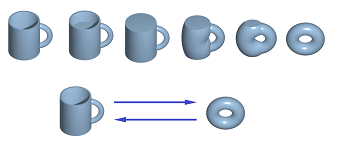
\includegraphics[scale=1]{mug-and-donut-homotopy-equivalence}
    \caption{Deformation of a coffee mug to donut showing the equivalence of both subspace of $\RR^3$}
\end{figure}
\item Any convex subset of a Euclidean space is homotopic to a point.
\end{enumerate}

\begin{lem}
    The relation $X \simeq Y$ is an equivalence relation on topological spaces.
\end{lem}

\begin{proof}
    Reflexive and symmetric properties are obvious. To show transitivity consider the maps
    \begin{center}
        \begin{tikzcd}
            X \arrow[r, bend left=30, "f"]
            \arrow[r, "g"', leftarrow,bend right=30]
            & Y
            \end{tikzcd}
\qquad
            \begin{tikzcd}
                Y \arrow[r, bend left=30, "u"]
                \arrow[r, "v"', leftarrow,bend right=30]
                & Z
                \end{tikzcd}
    \end{center} 
    which are homotopy equivalences, the by lemma (\ref{lem:hom-top-comp})
    \[
        g \circ v \circ u \circ f \simeq g \circ 1_Y \circ f = g \circ f \simeq 1_X  
    \]
    and 
    \[
        u \circ f \circ g \circ v \simeq u \circ 1_Y \circ v = u \circ v \simeq 1_Z  
    \]
    Therefore the maps
    \begin{center}
            \begin{tikzcd}
                Y \arrow[r, bend left=30, "u \circ f"]
                \arrow[r, "g \circ v"', leftarrow,bend right=30]
                & Z
                \end{tikzcd}
    \end{center}
    show that $X$ and $Z$ have the same homotopy type.
\end{proof}

\begin{defn}[Contractible space]
A space $X$ is called contractible if the identity map $1_X$ is homotopic to the constant map at some point of $X$.
\end{defn}

\section{Manifolds}
Before we give the definition of what a configuration space is we give some exposition of manifolds.
\begin{defn}[Manifold\cite{lavalle2006planning}]
    A topological space $M \subseteq \RR^m$ is a \textit{manifold} if for every $x \in M$, there exists an open set $O \subset M$ such that 
    \begin{enumerate}
        \item $x \in O$
        \item $O$ is homeomorphic to $\RR^n$
        \item $n$ is fixed for all $x \in M$
    \end{enumerate}
    The fixed $n$ is called the dimension of the manifold.
    \begin{figure}[H]
        \centering
        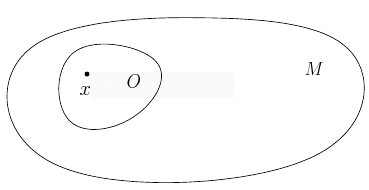
\includegraphics[scale=.95]{manifold}
    \end{figure}
\end{defn}

From the above definition, it is obvious that $m \ge n$ and it is impossible for a manifold to include its boundary points since they are not contained in open sets.
\linebreak
A manifold with boundary can be defined requiring that the neighborhood of each boundary point of $M$ is homeomorphic to a half-space of dimension $n$ and the interior points must be homeomorphic to $\RR^n$.

Now, we give presentation on the construction of some basic manifolds that frequently appear in motion planning.

\subsection{Examples of manifolds}

\begin{enumerate}
    \item \textbf{$1D$ manifolds}: A very obvious example of a one dimensional manifold is $\RR$, since by homeomorphism $\RR$ looks like $\RR$ in the vicinity of every point. The range can be restricted to the unit interval to yield the manifold $(0,1)$ since they are homeomorphic.

    Another example of a $1D$ manifold is a circle, say $\Sb^1$, where
    \[
        \Sb^1 = \{(x,y) \in \RR^2 \mid x^2 + y^2  = 1\}
    \]
    \item \textbf{$2D$ manifolds}: Many important $2D$ manifolds can be formed by applying cartesian product to $1D$ manifolds. 
    \begin{itemize}
        \item The $2D$ manifold $\RR^2$ is formed by $\RR \times \RR$ 
        \item The product $\RR \times \Sb^1$ defines a manifold that is equivalent to an infinite cylinder
        \item Also, $\Sb^1 \times \Sb^1$ is a manifold that is equivalent to a torus.
    \end{itemize}
    \begin{figure}[H]
        \centering
        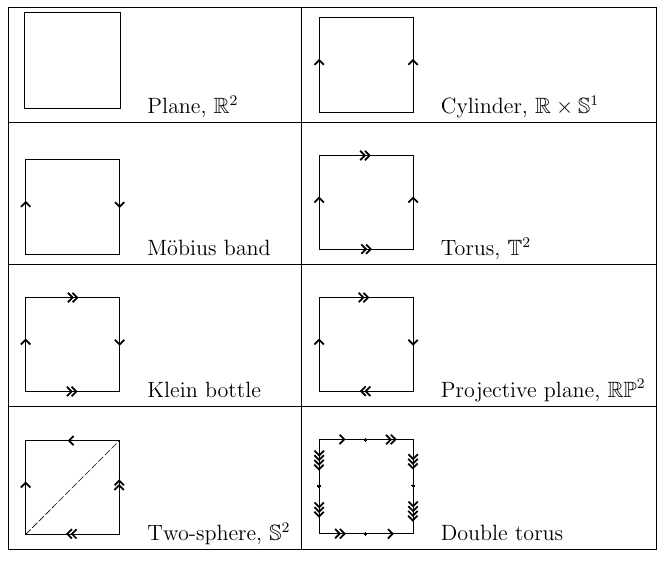
\includegraphics[scale=.7]{2d-manifolds}
        \caption[2D manifolds]{Some 2D manifolds that can be obtained by identifying pairs of points along the boundary of a square region\cite{lavalle2006planning}}
    \end{figure}
\end{enumerate}


\section{Fundamental Group}
\begin{defn}[Loop]
    Let $X$ be a topological space and $\gamma : X \lra [0,1]$ be a continuous path in $X$. We call $\gamma$ a \textit{loop} if $\gamma(0) = \gamma(1)$.
\end{defn}

\begin{defn}[Loop]\cite{enwiki:fg}
    Let $X$ be a topological space a loop at a based at $x_0$ is the continuous path $\disp \gamma : [0,1] \lra X$ such that the starting point $\gamma(0)$ and the end point $\gamma(1)$ are both equal to $x_0$
\end{defn}

Now, let $\alpha$ be a loop and let some $x_b$ be designated as a base point. For some arbitrary but fixed basse point, $x_b$, consider the set of all loops such that $\alpha(0) = \alpha(1) = x_b$. This can be made into a group by defining the following opeartion.

Let $\tau_1 : [0,1] \ra X$ and $\tau_2 : [0,1] \ra X$ be two loop paths with the same base point. We define their product as $\tau = \tau_1 \cdot \tau_2$ and is defined as
\begin{equation}\label{eqn:fgbo}
    \tau(t) = (\tau_1 \cdot \tau_2)(t) = \begin{cases}
        \tau_1(2t) & 0 \le t < \frac12 \\
        \tau_2(2t - 1) & \frac12 \le t \le 1
    \end{cases}  
\end{equation}

This results in a continuous loop path because $\tau_1$ terminates at $x_b$, and $\tau_2$ begins at $x_b$. That is the two paths are concatenated end to end.

Suppose now that the equivalence relation induced by homotopy is applied to the set of all loop paths through a fixed point, $xb$ . It will no longer be important which particular path was chosen from a class; any representative may be used. The equivalence relation also applies when the set of loops is interpreted as a group. The group operation actually occurs over the set of equivalences of paths.

The quotient set of the set of loops illustrated above and the equivalence class of homotopy form a group with respect to the binary operation $\cdot$ defined in (\ref{eqn:fgbo}) above and its construction is illustrated below. 

The identity element is the constant loop which stays at $x_b$ for all $t \in [0,1]$, inverse of a loop is the same loop but traversed in an opposite direction. That is $\tau^{-1}(t) = \tau(1-t)$. To show associativity, consider the three loops $\tau_0, \tau_1,\tau_2$, the products $\tau_0 \cdot (\tau_1 \cdot \tau_2)$ and $(\tau_0 \cdot \tau_1) \cdot \tau_2$ is the concatenation of the loops traversing $\tau_0$ to $\tau_1$ and to $\tau_2$. Though the concatenation is not in same order, but we are only considering the class upto homotopy, the loops are the same, then we have that:
\[
    (\tau_0 \cdot \tau_1) \cdot \tau_2 = \tau_0 \cdot (\tau_1 \cdot \tau_2)
\]
which shows that the quotient set of loops with base point $x_b$ with respect to the equivalence class of homotopy on $X$ is a group. Such group is called the \textit{fundamental group} of $X$ and it is denoted $\pi_1(X)$.

\subsection{Examples of Fundamental Groups}
\begin{enumerate}
  \item \textbf{Simply connected space}: Suppose that a topological $X$ is simply connected. In this case, all loop paths from a base point $x_b$  are homotopic, resulting in one equivalence class. The result is $\pi_1(X) = 1_G$, which is the group that consists of only the identity element\dots

  \item \textbf{The Fundamental group of a Circle}: Suppose $X = \Sb^1$. In this case, there is an equvalence class of paths for each $i \in \ZZ$, if $i > 0$, then it means  that the path winds $i$ times around $\Sb^1$ in the counterclockwise direction and then returns to $x_b$. If $i < 0$, then the path winds around $i$ times in the clockwise direction. If $i = 0$, then the path is equivalent to the one that remains at $x_b$. The fundamental group is $\ZZ$, with respect to the operation of addition. If $\tau_1$ travels $i_1$ times counterclockwise, and $\tau_2$ travels $i_2$ times counterclockwise, then $\tau = \tau_1 \cdot \tau_2$ belongs to the class of loops that travel around $i_1 + i_2$ times counterclockwise. Now to consider additive inverses, suppose a path travels ten times around $\Sb^1$, and it is combined with a path that travels ten times in the opposite direction, the result is homotopic to a path that remains at $x_b$. Thus, we have that $\pi_1(\Sb^2) = \ZZ$.
  \item \textbf{The fundamental group of Torus, $\TT$:} For the torus, $\pi_1(\TT^n) = \ZZ^n$, in which the $i$th component of $\TT^n$. The fundamental group $\ZZ^n$ is obtained by starting with a simply connected subset of the plane  and drilling out $n$ disjoint, bounded holes.
    \begin{figure}[H]
      \begin{center}
        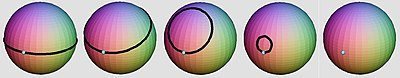
\includegraphics[width=0.85\textwidth]{sphere-homo}
      \end{center}
      \caption{A loop on a $2$-sphere (the surface of a ball) beiing contracted to a point \cite{enwiki:fg}
}
    \end{figure}
\end{enumerate}
The table below gives a summary of some space and the fundaental groups.
\begin{table}[H]
  \centering
  \begin{tabular}{c|c}
    \hline
    Space & Fundamenta group \\
    \hline 
    Convex subset of $\RR^n$ & Trivial \\
    Circle & $\ZZ$ \\
    $\Sb^n, n \ge 2$ & Trivial \\
    Torus ($\TT^n$) & $\ZZ^n$ \\
    Klein bottle & $\{a, b \mid a^2 = b^2\}$
    \end{tabular}
\end{table}

More generally we give the following definition:

\begin{defn}\cite{mamouni2022pure}
   Let $X$ be a path-connected topological space, and $n$ a fixed integer. The $n$-homotopy group of $X$ is defined to be 
   \[  
      \pi_n(X) := \map(\Sb^n, X) / F
   \]
   where, $F$ is homotopy on $X$, $\Sb^n$ is the unit sphere of $\RR^{n+1}$, and $\map(\Sb^n, X) / F$ the quotient set of continuous maps $\gamma: \Sb^n \lra X$, upto homotopy.
\end{defn}

% \section{Configuration Space}
% There is no way we can discuss the application of topology to robotics without discussing the configuration space, since that is the entry point of topology into the field of robotics.
